%%%%%%%%%%%%%%%%%%%%%%%%%%%%%%%%%%%%%%%%%
% Twenty Seconds Resume/CV
% LaTeX Template
% Version 1.1 (8/1/17)
%
% This template has been downloaded from:
% http://www.LaTeXTemplates.com
%
% Original author:
% Carmine Spagnuolo (cspagnuolo@unisa.it) with major modifications by
% Vel (vel@LaTeXTemplates.com)
%
% License:
% The MIT License (see included LICENSE file)
%
%%%%%%%%%%%%%%%%%%%%%%%%%%%%%%%%%%%%%%%%%

%----------------------------------------------------------------------------------------
%	PACKAGES AND OTHER DOCUMENT CONFIGURATIONS
%----------------------------------------------------------------------------------------

\documentclass[letterpaper]{twentysecondcv} % a4paper for A4

\usepackage[super]{nth}
\usepackage{enumitem}

\definecolor{OliveGreen}{rgb}{0,0.5,0.1}

\hypersetup{colorlinks,urlcolor=blue!50!black}

\newcommand{\myhy}[2]{\underline{\href{#1}{#2}}}

\setitemize{noitemsep,topsep=0pt,parsep=0pt,partopsep=0pt}

%----------------------------------------------------------------------------------------
%	 PERSONAL INFORMATION
%----------------------------------------------------------------------------------------

\profilepic{}

\cvname{Ramses A.}
\cvjobtitle{Networks Engineer}

\cvdate{} % it is preferred not to put your age in Canada
\cvaddress{\vspace{-12px}
           Montreal, Quebec\newline
           Permanent Resident of Canada}
\cvnumberphone{+1 343-777-4060}
\cvmail{\myhy{mailto://admin@ramses.ca}{admin@ramses.ca}}
\cvsite{\myhy{https://ramses.ca}{ramses.ca}}
\cvlinkedin{\myhy{http://www.linkedin.com/in/mabdelaz/}{linkedin.com/in/mabdelaz}}

%----------------------------------------------------------------------------------------

\begin{document}

%----------------------------------------------------------------------------------------
%	 ABOUT ME
%----------------------------------------------------------------------------------------

\aboutme{I am a Computer Engineer specialized in Network Systems, Data Centre Operations,
         Embedded Systems, and Computer Architecture. I am a Permanent Resident of Canada,
         and I can travel abroad if needed.
         \\
         %\vspace{10px}
        }

%----------------------------------------------------------------------------------------
%	 Technologies
%----------------------------------------------------------------------------------------

\tech{
    \center{
        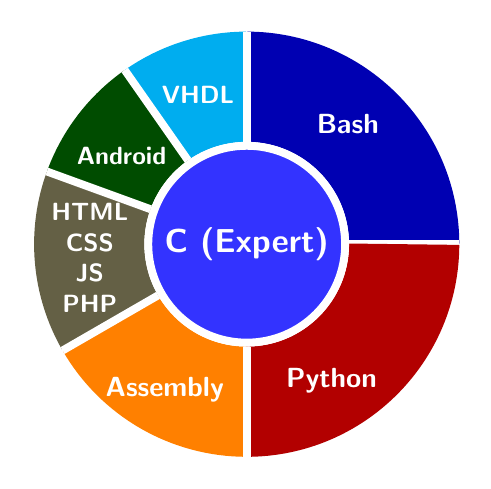
\begin{tikzpicture}[font=\sffamily\bfseries\large, text=white, border/.style={line width=14mm}]
        \foreach \angle/\col [remember=\angle as \last (initially 0)] in
            {90/blue!70!black, 125/cyan, 160/green!30!black, 210/yellow!30!black, 270/orange, 360/red!70!black}{
                \draw[\col, border] (\last:2cm)
                     arc[start angle=\last, end angle=\angle, radius=2cm];
                \draw[white, line width=1mm] (\last:1.3)--++(\last:1.4);
        }
        \node[line width=1mm, draw, circle, minimum width=2.5cm, white, fill=blue!80] {C (Expert)};
        \node[text width=1cm, align=center, font=\sffamily\bfseries\normalsize] at (50:2cm)  {Bash};
        \node[text width=1cm, align=center, font=\sffamily\bfseries\small] at (108:2cm) {VHDL};
        \node[text width=1cm, align=center, font=\sffamily\bfseries\small] at (146:2cm) {Android};
        \node[text width=1cm, align=center, font=\sffamily\bfseries\small] at (185:2cm) {HTML CSS JS PHP};
        \node[text width=1cm, align=center, font=\sffamily\bfseries\normalsize] at (235:2.25cm) {Assembly};
        \node[text width=1cm, align=center, font=\sffamily\bfseries\normalsize] at (300:2cm) {Python};
        \end{tikzpicture}
    }
}

%----------------------------------------------------------------------------------------
%	 OS PREFERENCES
%----------------------------------------------------------------------------------------

\ospref{
    \textcolor{black}{
    \textbf{Linux Administration}\hfill
\includegraphics[scale=0.40]{5stars.png}\newline
    \textbf{Network Deployment}\hfill
\includegraphics[scale=0.40]{5stars.png}\newline
    \textbf{Network Troubleshooting}\hfill
\includegraphics[scale=0.40]{5stars.png}\newline
    \textbf{Cisco H/W}\hfill
\includegraphics[scale=0.40]{5stars.png}\newline
    \textbf{Windows}\hfill
\includegraphics[scale=0.40]{3stars.png}}}

%----------------------------------------------------------------------------------------
%	 LANGUAGES
%----------------------------------------------------------------------------------------

\langs{
    \langlist{English     (\textit{Preferred})  }{}{6}
    \langlist{French      (\textit{Learning})   }{}{1}
    \langlist{Italian     (\textit{Basic})      }{}{2}
    \langlist{Hieroglyphs (\textit{Hobbyist})   }{}{0.5}
}

%----------------------------------------------------------------------------------------
%	 COURSES
%----------------------------------------------------------------------------------------

\courses{
    Academic Course Highlights: Programming, OOP, Software Engineering,
    Data Mining, AI, Data Structures, File Organization, Databases,
    Algorithm Analysis, OS, Compilers, Computer Architecture, Embedded
    Systems, and Networks.
}

%----------------------------------------------------------------------------------------

% Print the sidebar
\makeprofile

%----------------------------------------------------------------------------------------
%	 EDUCATION
%----------------------------------------------------------------------------------------

\section{Education}

\begin{twenty} % Environment for a list with descriptions
	%\twentyitem{<dates>}{<title>}{<location>}{<description>}
	\twentyitem{2011 - 2016}
               {B.Sc., Computer and Systems Engineering}
               {Alexandria University}
               {\textbf{Rank}: 1st (highest GPA)\newline
                \textbf{GPA}: 3.94/4.00\newline
                \textbf{Graduation Project}: \myhy{https://github.com/iocoder/graduation}
                                             {\textbf{FPGA} computer based on \textbf{MIPS} architecture}
                %\textbf{Course Highlights}: Control Theory, Modern Control, Embedded Systems,
                %                            Computer Architecture, Software Engineering,
                %                            System Software, Operating Systems, Compilers, Switching Theory,
                %                            Automata Theory, Complexity Theory.
               }
	%\twentyitem{2008 - 2011}
        %      {High School}
        %      {Mubarak Secondary School}
        %      {\textbf{Overall Grade}: 407.5/410 (99.36\%).\newline
        %       \textbf{Specialization}: Mathematics.}
\end{twenty}

%----------------------------------------------------------------------------------------
%	 Highlights
%----------------------------------------------------------------------------------------

%\section{Highlights}

%\begin{itemize}
%    \item{Confident, friendly, very polite, and always smiling when
%          dealing with customers and co-workers.}
%    \item{Excellent interpersonal and communication skills in \textbf{English}.}
%    \item{Great ability to learn new technologies quickly.}
%    \item{Advanced technical writing skills in \textbf{\LaTeX} (this r\'esum\'e is an example).}
%    \item{Extensive knowledge of the foundations of Computer Science.}
%\end{itemize}

%----------------------------------------------------------------------------------------
%	 EXPERIENCE
%----------------------------------------------------------------------------------------

\section{Experience}

\begin{twenty}

\twentyitem{\hspace{2ex} Current}
           {\underline{Networks Engineer at \textcolor{OliveGreen}{Cisco}, Ottawa}}
           {}
           {\\
            My team works on a number of crucial features for \textbf{Cisco 8000 Series},
            \textbf{NCS5000 Series}, and \textbf{ASR9K Family} to satisfy Service Provider
            market needs. I also contributed to \textbf{Cisco Catalyst} and \textbf{Nexus 9000}.
            My daily tasks included:
            \\
            \begin{enumerate}
               \item{Implementing new components for \textbf{Cisco's IOS/XR}, \textbf{IOS/XE}, and \textbf{NXOS} Operating Systems in C.}
               \item{\textbf{Designing and deploying} new \textbf{testbeds} and laying out new racks in our internal \textbf{data centres and labs}.}
               \item{Utilizing my \textbf{Linux Expertise} to administer the data centre.}
               \item{Developing a decent \textbf{automation} platform to assist my team with automating integration testing (\textbf{bash/python}).}
               \item{Enhancing our use of \textbf{virtualization technologies}, including \textbf{vSphere}, \textbf{KVM}, etc.}
               \item{\textbf{Troubleshooting} network problems and fixing failed routers.}
               \item{Writing \textbf{Documentation} and Specifications for my work.}
               \item{\textbf{Training} new hires and interns on Networking/OS basics and Cisco products.}
            \end{enumerate}
           }

  \twentyitem{\hspace{2ex} 2018}
             {\underline{Software Engineer at \textcolor{OliveGreen}{SoundHound}, Toronto}}
             {}
             {\\
              Working with a team of top-notch AI engineers on high-end Speech Recognition and Natural Language Processing products. Some of the job responsibilities included:
              \\
              \begin{enumerate}
                 \item{Leveraging my \textbf{C/C++} programming skills to develop server-side \textbf{NLP} modules.}
                 \item{Provide \textbf{Linux} technical expertise to the automation of various processes.}
                 \item{Manipulating and managing large database systems.}
              \end{enumerate}
             }

	\twentyitem{\hspace{2ex} 2017}
               {\underline{Researcher (Networks) at \textcolor{OliveGreen}{Simon Fraser University}, Vancouver}}
               {}
               {\\
                Implementation of an LTE base station using \textit{Ettus B210} \textbf{USRP} (\textbf{Software-Defined Networking}) and \textit{OpenAirInterface}.
               }

	%\twentyitem{\hspace{2ex} 2017}
    %           {\underline{Control Systems Engineer at \textcolor{OliveGreen}{Advanced HVAC Consultant}, Cairo}}
    %           {}
    %           {Implementation of feedback control loops for \textbf{HVAC} systems using \textit{Fupla} (function block diagrams) on
    %            \textit{Saia Burgess} \textbf{PLC} devices.

                %\\ The work included.
                %\begin{enumerate}
                %   \item{Control loops for airhand units (fans, valves, and sensors).}
                %    %\item{Control loops for chillers and water pumps.}
                %    \item{Interfacing \textit{Saia Burgess PLCs} and \textit{Honeywell Eagle DDCs} using
                %          \textbf{Modbus} and \textbf{Bacnet/IP}.}
                %    %\item{Developing interactive Human-Computer Interfaces using \textit{Tridium controller}
                %    %      to interface the human operator with PLC logic.}
                %    \item{Instructing our teams on the implementation of electrical boards composed of
                %          \textbf{high-voltage relays} and networks of PLCs.}
                %    %\item{Troubleshooting and solving technical problems at the field.}
                %\end{enumerate}
     %          }

	%\twentyitem{\hspace{2ex} 2016}
    %           {\underline{Software Engineer at \textcolor{OliveGreen}{Ejada Systems}, Alexandria}}
    %           {}
    %           {Providing enterprise solutions to banks in the Middle East, including:
    %            \begin{enumerate}
    %                \item Implementation of \textbf{CRM} systems using \textbf{Oracle Siebel}.
    %                \item Developing \textbf{BigData} solutions using
    %                      \textbf{Hadoop} and \textbf{Scala}.
    %            \end{enumerate}}

	\twentyitem{\hspace{2ex} 2015}
               {\underline{RA Intern (Networks) at \textcolor{OliveGreen}{SmartCI Research Center}, Alexandria}}
               {}
               {\\
                Programming the storage system of a cognitive radio cloud, which consisted of
                Linux nodes with \textbf{ext2fs}, using \textbf{IP multicast} and \textbf{filesystem-aware}
                \textbf{data compression}.}

	%\twentyitem{<dates>}{<title>}{<location>}{<description>}
\end{twenty}

%----------------------------------------------------------------------------------------
%	 PUBLICATIONS
%----------------------------------------------------------------------------------------

\section{Selected Projects}

\begin{itemize}
    %\item{Expanada: Financial management application in \textbf{\underline{Python}} and \textbf{\underline{SQL}}.}
    %\item{XMLCurses: \textbf{\underline{Python library}} for programming libcurses applications using XML.}
    \item{Network system for OS image distribution over \textbf{{cloud network}} using Frisbee.}
    \item{\myhy{https://github.com/iocoder/wncp}{Radio KAOS}: \textbf{{Cognitive Radio Network}} with Dynamic Spectrum Sharing.}
    \item{CDP: \textbf{{Linux kernel driver}} implementation for a reliable Data Transfer Protocol.}
    \item{\myhy{https://github.com/quafios/quafios}{Quafios}:
          An \textbf{{Operating System}} for x86 and MIPS.
          %The system included:
          %\begin{itemize}
          %  \item Implementation of a UNIX-like \textbf{{system call}} interfaces.
          %  \item \textbf{{Device drivers}} for PCI, USB, ATA, timers, interrupt controller,
          %        keyboard controller, and other hardware components.
          %  \item Dynamic kernel-space and user-space \textbf{{memory allocation}} algorithms.
          %  \item Implementation for \textbf{{C library}} routines.
          %  \item A GUI, with a programmer-friendly API.
          %\end{itemize}
          }
    %\item{\textbf{{Compiler}} for a subset of \textbf{{C}} and
    %      \textbf{{Java}} Programming Languages}
    \item{Designed a \myhy{https://github.com/iocoder/cs333_f16_lab2/raw/master/CS333_F16_Lab2.pdf}{Linux kernel device driver and synchronization assignment}
          for OS course at Alexandria University.}
    %\item{Liftroid: Visualized elevator Android interface with \textbf{{AVR}}.}
    \item{\myhy{https://github.com/iocoder/uefi_report/raw/master/final_report.pdf}{Technical Report on Unified Extensible Firmware Interface}
          (\textbf{{UEFI}}).}
    %\item{Systema: Educational system-level \textbf{{programming language and compiler}}.}
    %\item{IDE to USB interface using AVR and PIC.}
    %\item{8086 micro-computer system.}
    %\item{Relational \textbf{\underline{Database}} Management System in \textbf{\underline{Java}}.}
    %\item{NES (Nintendo Entertainment System) Simulator.}
    %\item{Hello World \textbf{{BIOS}}.}
    %\item{Static RAM with MOSFETs on PCB.}
    %\item{T-DEC/102, a simulated TTL computer.}
    %\item{Educational Program with Animated Agent for Disabled Children in \textbf{\underline{VB.NET}}.}
\end{itemize}

%----------------------------------------------------------------------------------------
%	 AWARDS
%----------------------------------------------------------------------------------------

%\section{Selected Awards}
%
%\begin{twentyshort}
%	\twentyitemshort{2017}       {CSED Golden Armor for the \textbf{Top Student} of 2015-2016 Class.}
%	\twentyitemshort{2017}       {Prof. Naeem Abou Taleb Award for \textbf{Top Student}.}
%	\twentyitemshort{2012 - 2016}{\textbf{Certificate of Excellence}, Alexandria University.}
%	%\twentyitemshort{<dates>}{<title/description>}
%\end{twentyshort}

\vfill
\footnotesize{
\begin{itemize}[leftmargin=10px]
    \item[--] You can find the \LaTeX source code of my resume at \color{blue}{
                 \myhy{http://www.github.com/iocoder/resume}{http://www.github.com/iocoder/resume}}.
\end{itemize}
}

\end{document}
